\subsection{Dual Ecological Measures of Focus in Software Development\\ \textit{D. Posnett, R. D’Souza, R. Devanbu, V. Filkov\\ 2013 - ICSE}}

This paper took an interesting approach to measuring the relation between component and developer. Using a biological analogy with prey/predator type relationships between components and developers. That is to say that modules prey on a developer's time. Therefore, in this visualisation, we have two points of view. On the one hand, the developers, and the contributions they have made to each component (a larger edge represents more contributions), and on the other hand, we have the components, and the contributions they have received. As in the following figure:

\begin{figure}[H]
\centering
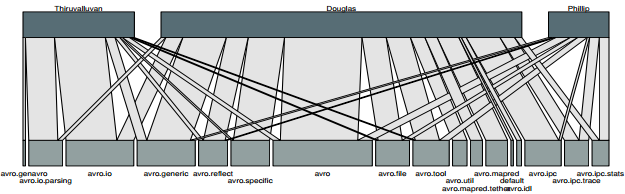
\includegraphics[width=0.5\textwidth]{./resources/focus.png}~
\caption{Ownership map By Feature}
\label{fig:ownership_map_by_feature}
\end{figure}

This paper evokes the notion of Focus, both from the developers' point of view and the components'.
\\[0.4cm]
\textbf{DAF: Developer’s Attention Focus}
\begin{itemize}
\item Human attention and cognition are finite resources. If they are spread across many tasks, we can usually see a degradation in performance, and errors, and thus the quality of work will suffer. This is the same with all things, and especially in software development.
\item This metric is designed to measure how focused a developer is on his work, and thus give an indication of the quality of his work compared to his potential.
\end{itemize}

\textbf{MAF: Module Activity Focus}
\begin{itemize}
\item Measures the degree to which activities on the component are focused.
\end{itemize}

Components are viewed as predators, which hunt developers' cognitive resources. When there is a large amount of contributors on a component, it can "feed" and thus thrive.
Developers are viewed as prey, whose limited cognitive ressources are divided amoung the components that are "hunting" them.

Therefore, a developer with a high amount of commits on a single component will have higher focus, whereas a developer with a large amount of commits on several components will have lower focus.
This gives us an idea of the limitations of ownership, because in the second case, the developer might still be considered as owner of several modules, without having concentrated his efforts on these modules.

However, a developer may have high concentration on a few files in a component, but only made small contributions when compared to other developers working on the same module.
Also, a developer that contributes a few times on a large/popular component will not be as specialised as a developer which has made as many contributions to a smaller component.

Given this information, there a some questions to be raised:
\begin{itemize}
\item What kind of behavioural pattern do the top developers follow?
\item Is there any correlation between a high focus and a low amount of bugs?
\end{itemize}

\textbf{Conclusions:}
\begin{itemize}
\item Project leaders tend to have lower levels of Focus than other Developers.
\item High focus implies less bugs introduced.
\item Increasing the Module Activity Focus (MAF) has a negative impact on the quality of that module.
\end{itemize}

This paper and it's visualisation is what inspired us the most when deciding what kind of visualisation we should create.